\normaltrue
\correctionfalse

%\UPSTIidClasse{12} % 11 sup, 12 spé
%\newcommand{\UPSTIidClasse}{12}

\exer{Question de cours -- Flexion $\star$ \label{RDM:04:flx:539:cours}}
\setcounter{question}{0}\marginnote{\xpComp{RDM}{04}}%\UPSTIcompetence[2]{C2-10}
\index{Compétence RDM-04}



\ifcorrection
\else
\marginnote{\textbf{Pas de corrigé pour cet exercice.}}
\fi


\question{Donner la définition de la contrainte en flexion et l'équation de la déformée. Donner la contrainte de cisaillement.}
\ifprof
$\sigma = -\dfrac{M_{fz}}{I_{Gz}}y$, $M_{fz}= EI_{Gz}y''(x)$.

$\tau = \dfrac{T_y}{S}$.
\else
\fi

\question{Donner la défintion du moment quadratique. Calculer $I_{Gz}(S)$ pour une poutre creuse de section circulaire (grand rayon $R$ et petit rayon $r$).}
w
\ifprof
$I_{Gz}(S) = \int_S y^2 \dd S$
\else
\fi

\question{Tracer le champ de contrainte dans une poutre creuse de section circulaire en flexion simple. }
\ifprof
\else
\fi


\begin{marginfigure}
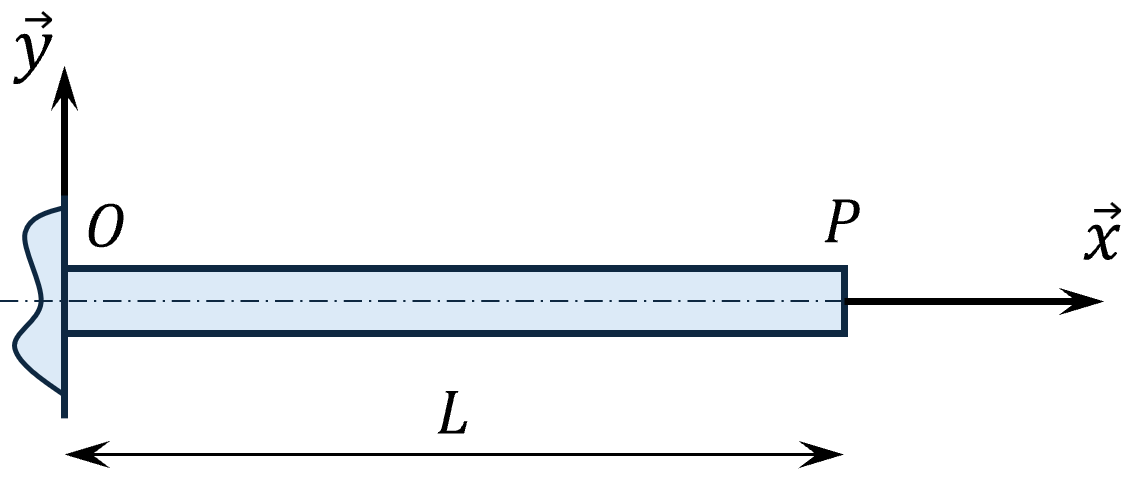
\includegraphics[width=\linewidth]{539_01.png}
\end{marginfigure}

Dans le chargement ci-contre, on donne $L = \SI{1}{m}$, $F=\SI{100}{N}$. La poutre est creuse, de section cylindrique est de diamètre \SI{10}{mm}.


\question{Déterminer le torseur de cohésion dans la poutre.}
\ifprof
\else
\fi

\question{Déterminer la contrainte normale maximale.}
\ifprof
\else
\fi

\question{Donner l'équation de la déformée et la représenter.}
\ifprof
\else
\fi


\question{Déterminer la flèche maximale de la poutre.}
\ifprof
\else
\fi

%\question{La poutre est remplécée par une poutre cylindrique à une poutre creuse de diamètre extérieur \SI{10}{mm} et de diamètre intérieur de \SI{5}{mm}.}
%\ifprof
%\else
%\fi


\ifprof

\else
%\footnotesize
%\begin{enumerate}
%  \item $\left(fp + Mp^2\right) Z(p)=S_h P_h(p)-S_e P_e(p) - \dfrac{Mg}{p}$
%    \item $Q_e(p)=\left(S_a - S_b \right)pL(p) + \dfrac{V_t}{B_e} p P_e(p)$ et $mp^2 L(p) = -rL(p)+\left(S_a-S_b\right) P_e(t)-f'pL(p)$.
%\end{enumerate}
%\normalsize

\marginnote{Corrigé voir \ref{RDM:04:flx:539:cours}.}

\fi